
\documentclass[]{spie}

% Package imports go here.
\renewcommand{\baselinestretch}{1.0} % Change to 1.65 for double spacing

\usepackage{amsmath,amsfonts,amssymb}
\usepackage{graphicx}
\usepackage[colorlinks=true, allcolors=blue]{hyperref}
\usepackage{listings}
\usepackage{xcolor}
\usepackage{longtable}

% Local commands go here.
\newcommand{\aj}{AJ}
\newcommand{\apj}{ApJ}
\newcommand{\apjs}{ApJS}
\newcommand{\procspie}{Proc.\ SPIE}
\newcommand{\pasj}{PASJ}
% lsstdoc documentation: https://lsst-texmf.lsst.io/lsstdoc.html
\input{meta}

% Package imports go here.

% Local commands go here.

% See ASPmanual2010.pdf 2.1.4  and ManuscriptInstructions.pdf for more details
%\markboth{auth}{short title}


\newcommand{\docRef}{RTN-081}
\newcommand{\docUpstreamLocation}{\url{https://github.com/lsst/rtn-081}}


\begin{document}
\input{authors}
\title{Rubin Observatory Operations: Enabling collaborative ground-up budget planning across a multi-team organization}

% This can write metadata into the PDF.
% Update keywords and author information as necessary.
\hypersetup{
    pdftitle={Rubin Observatory Operations: Enabling collaborative ground-up budget planning across a multi-team organization},
    pdfauthor={petryce},
    pdfkeywords={}
}

\maketitle


\begin{abstract}
Change is inevitable in large big budget operational programs. Embracing, rather than resisting, change is key to being proactive. It also keeps teams motivated as it’s another avenue for leadership to “listen” to what is going on at the team level. At Rubin Observatory an agile approach to budgeting has been implemented. Annually a bottom up review to address changing needs, priorities and emerging issues, called a scrub, is carried out across all departments of the Rubin Operations organization. This provides an opportunity to adapt and be nimble to changing situations that can affect resources and budgets. This paper will provide details on the importance for an annual budget scrub, processes followed, tools used, and how the cycle continues year on year.
\end{abstract}





\section{Introduction} \label{sec:intro}
Vera C. Rubin Observatory\cite{2008arXiv0805.2366I} is currently under construction. 
Once complete, the observatory will consist of an end to end system with the mountain top Summit Facility on Cerro Pachon in Chile housing an 8.4m telescope and a 3200 megapixel camera, a high bandwidth long haul network, a system of data processing facilities in California, France and the UK, a data management system, a data access platform in the cloud, and a host of public engagement programs. 
Naturally this means the observatory is distributed across a number of locations. 
The observatory is due to start full operations in 2025; the survey will be carried out over a period of ten years, and a post-operations phase will follow. 
The operation of Rubin Observatory is fairly unique in astronomy for being funded in approximately equal shares by two US government agencies, and operated by two almost equal partner national laboratories (NSF's NOIRLab and SLAC National Accelerator Laboratory, funded by the Department of Energy). 
Budgets are usually set at high level years in advance, but things rarely stay the same.
This paper describes an annual ground-up budgeting process adapted from the one used by the US-ATLAS operations team, in support of the ATLAS experiment at the Large Hadron Collider at CERN. 
The aim of this annual exercise is to enable change within the budget envelope.
The paper provides the reader with details of all the tools that are used, and describes the process that is followed annually.

\section{Process} \label{sec:process}


Throughout the Rubin pre-operations and operations phases, annually in May each team will look back at what was planned, what was achieved, do a full review of its activities, and propose a high level plan for the following (US fiscal) year.
This is standard practice in other high energy physics experiments as well, the scrub allows the facility to continuously evolve its operating plan, taking critical input from the people that understand best what is really needed, in Rubin’s case that is the Team Leaders.
Following the National Science Foundation and Department of Energy joint annual review of Rubin Operations the Rubin Operations Directors office together with department heads sets the major milestones for the next US fiscal year (FY) starting 1st October. This includes looking at the status of major milestones for the current year and ascertaining whether any of those need to carry over into the next FY.
With the major milestones set, the Director’s office kicks off the month long annual scrub process, see \autoref{fig:timeline} in which the department heads start down stream planning with their teams. This is the “homework” phase of the scrub where teams are looking at:

\begin{itemize}
\item status of minor milestones for the current FY
\item setting minor milestones that would contribute to accomplishing the new major milestones for the next FY
\item based on activities needed to achieve the minor milestones and risk mitigation plans the teams review planned resources both labor and non-labor
\item if there is a mismatch between resources needed and the resources available the team will propose changes during this scrub period through the tool (described in the next section).

\end{itemize}


\begin{figure}[hb!]
\begin{centering}
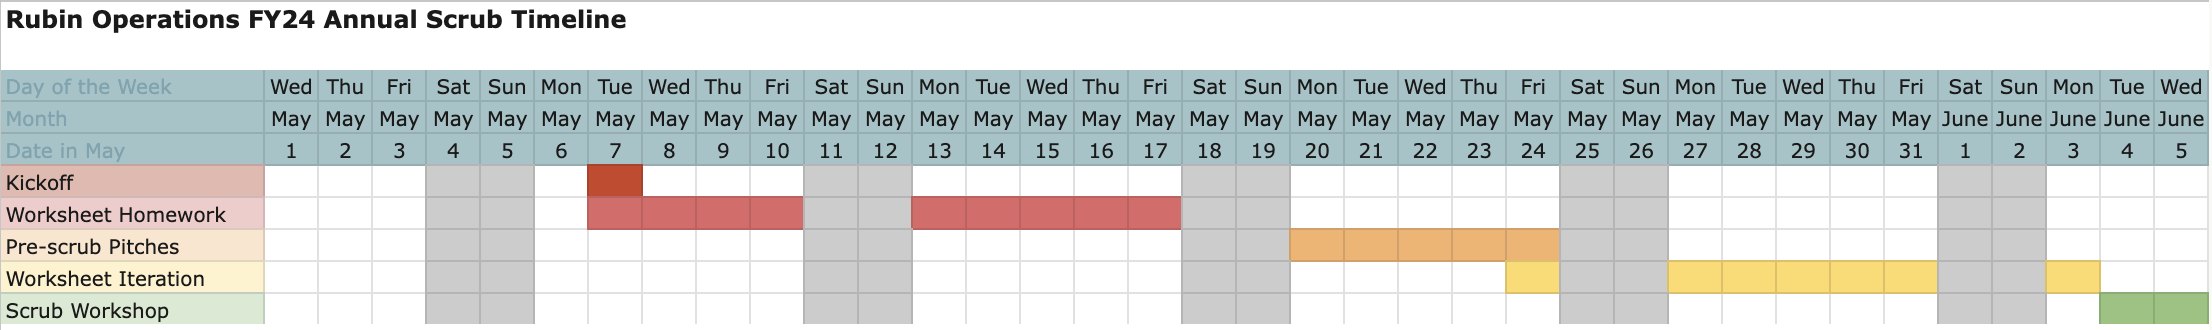
\includegraphics[width=1.0\textwidth]{Figure1Scrubtimeline}
	\caption{Scrub timeline
\label{fig:timeline}}
\end{centering}
\end{figure}
Having completed the above homework, in the tool provided, the scrub moves into the “pitches” phase. Department heads and team leads prepare short presentations, for which a template is provided, to pitch the needed changes to the Director’s office. As additional resource requests from one department could impact another, all department leads and team leads are invited and encouraged to attend all pitches. Currently in Rubin the 15-30 minutes team level pitches are carried out per department in virtual format. This is in contrast to the ATLAS Experiment where the teams come together for an in-person gathering to present pitches.

After the pitches phase is complete a period of iteration takes place between the director’s office and department/team to reach an agreement on the changes.

The directors office is aggregating the labor and non-labor baseline vs proposed changes across the Rubin departments to ensure the program remains overall within the defined financial envelope. This is one of the reasons for the back and forth iterations and negotiations as priorities have to drive this process.

After agreement the changes are implemented by propagating them throughout the Rubin planning tools culminating in the spending plan for the next FY and definition of Statements of Work for the contracts enabling requisitions to be input in time for contracts to be placed.

With the resources now updated across all the tools teams can start realistically planning for the coming FY by defining the tasks and activities that will lead to completion of the defined minor milestones within the boundaries of the available resources. Work then commences at the start of the FY. The activity planning is done in an Atlassian tool called Jira where the milestones are defined enabling downstream and upstream traceability between milestones to tasks.The Jira tool is outside the scope of this paper.

From the start of the FY the Director’s office takes inputs, such as overhead rates, escalation rates etc, as defined by the managing organization and preps the tools for the next annual scrub and so the cycle continues, see see \autoref{fig:cycle}.


\begin{figure}
\begin{centering}
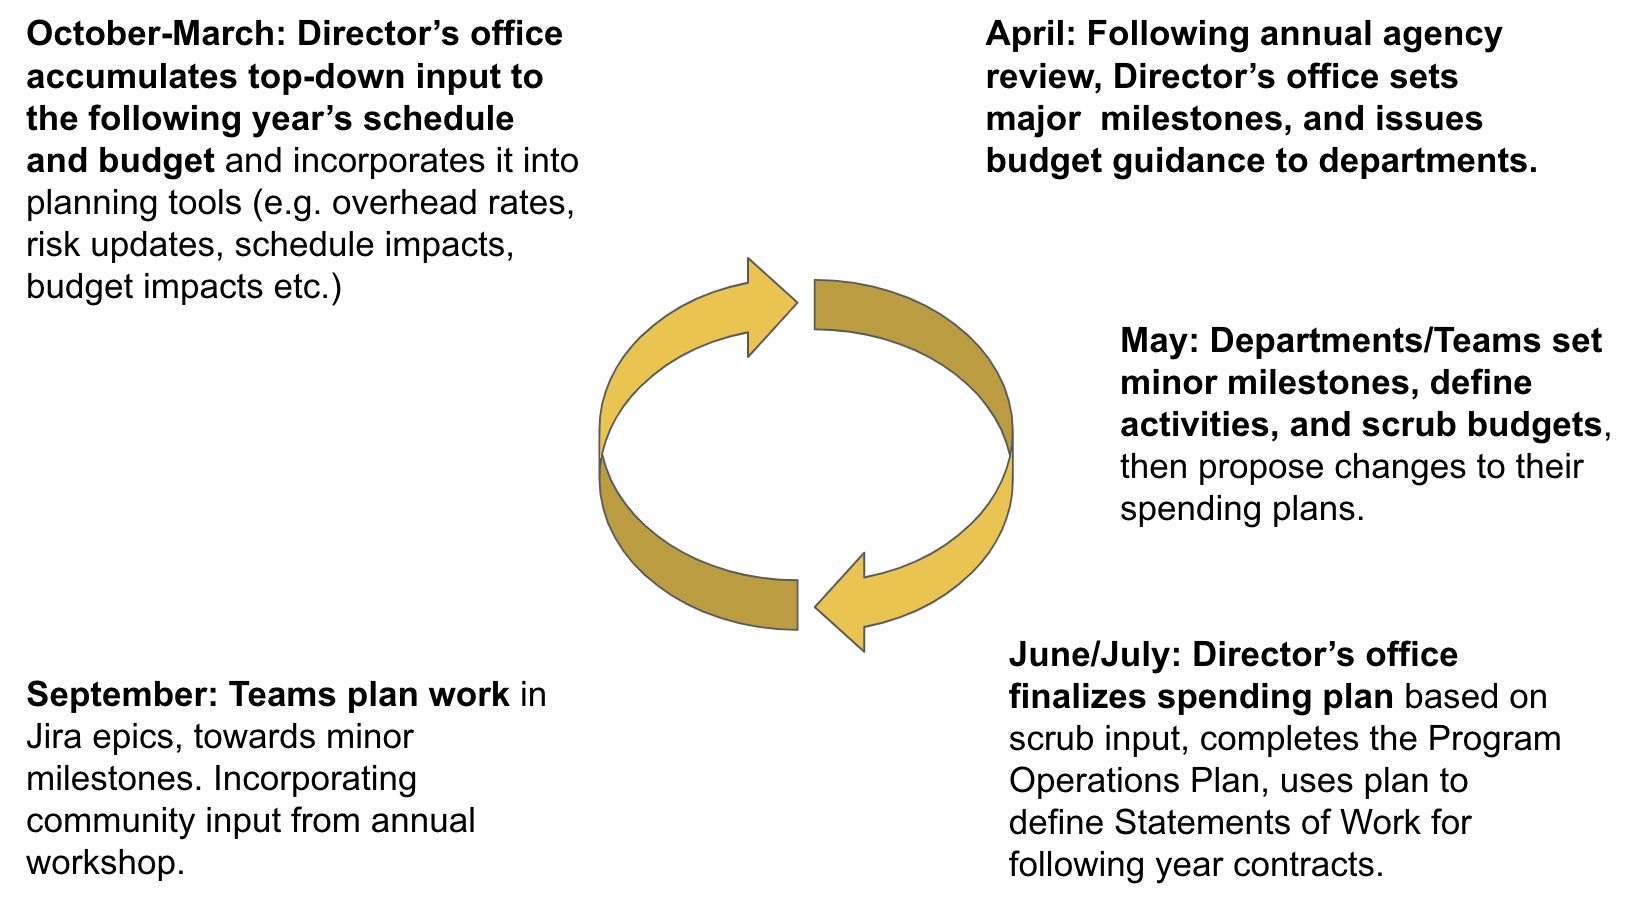
\includegraphics[width=1.0\textwidth]{Figure2AnnualPlanningScrubCycle}
	\caption{The annual planning and scrub cycle
\label{fig:cycle}}
\end{centering}
\end{figure}

\section{Tools} \label{sec:tools}

This section describes the tools used for the scrub process. 
With the requirement for agility, collaborative working and ease of linking to existing tools, Google Workspace is the chosen platform on which all the Rubin planning tools, including the scrub tool, have been developed. 
The particular tool that supports the annual scrub is a Google Sheets workbook called the ``Scrub Sandbox.''
It needs to facilitate:
\begin{enumerate}
\item capturing the current state of the operations plan for each team;
\item capturing what the desired changes are;
\item inputting flow down milestones for the upcoming FY based on higher level milestones defined by the directors Office;
\item standardizing inputs coming in from the Departments and Teams;
\item easiy visualization of the impact of the desired change on the labor and non-labor budgets;
\item collaboration between Team Leaders as they work through their competing needs.
\end{enumerate}

\begin{figure}[h!]
\begin{centering}
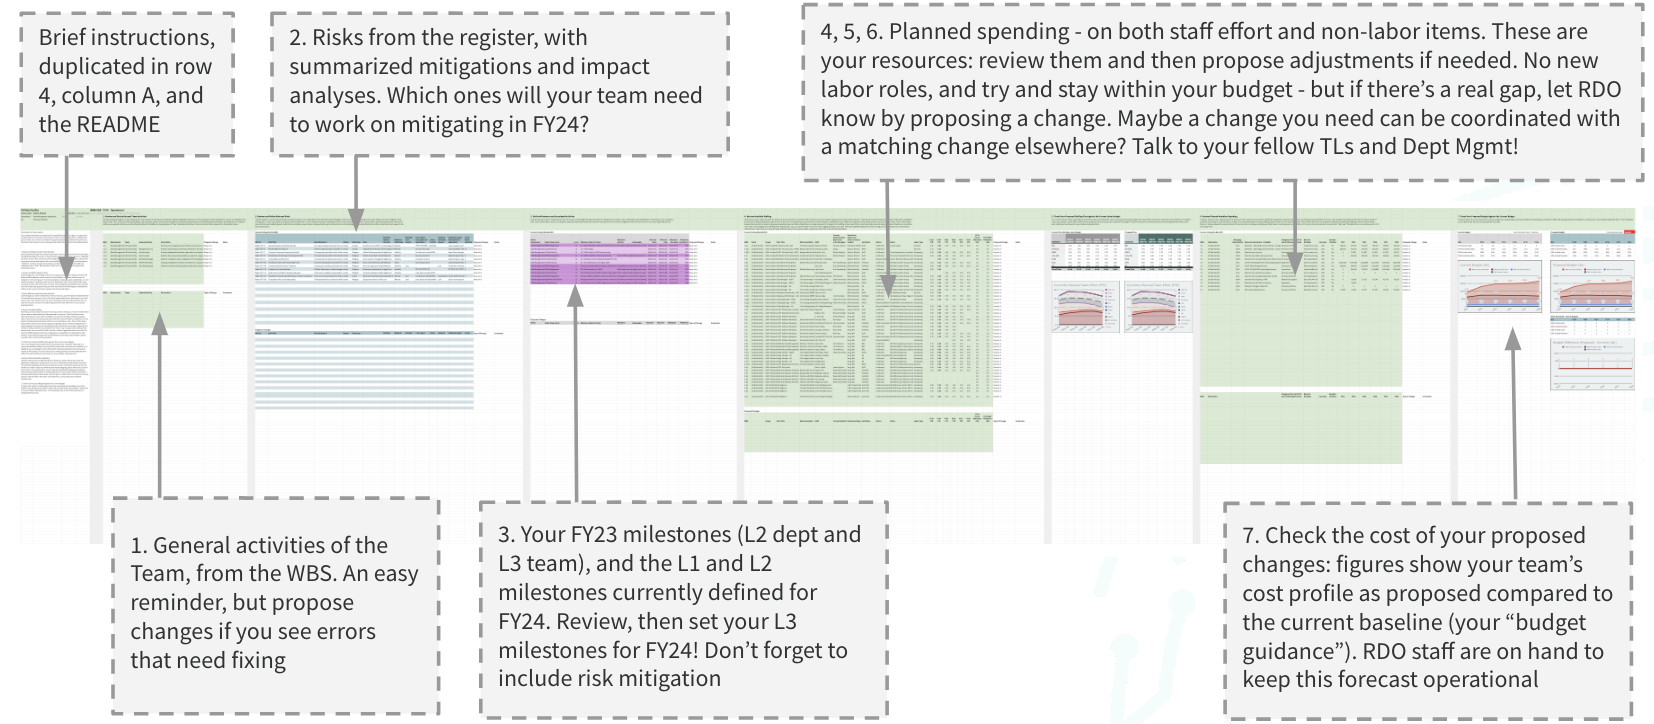
\includegraphics[width=1.0\textwidth]{Figure3OverviewScrubSandbox}
	\caption{ Overview of the Scrub Sandbox tool.
\label{fig:sandbox}}
\end{centering}
\end{figure}

\noindent Furthermore, the tool needs to enable the following aspects of the overall operations plan to be scrubbed:
\begin{enumerate}
\item Work Breakdown Structure (WBS);
\item Risks;
\item Milestones;
\item Labor expenditure;
\item Non-labor expenditure.
\end{enumerate}
Each Team is provided with a sheet within the workbook, that follows a standard layout. 
The worksheet is organized into 7 vertical sections, where the left to right flow is through each of the aspects in the above list. 
Within all sections of all worksheets, the tool implements a standard approach to the proposing of changes (see \autoref{fig:wbs}).
An upper block of cells displays the current plan for that aspect, imported dynamically from the relevant planning tool using the \texttt{importrange} command (e.g. the vital information for the risks assigned to a team are read in from the Risk Register).
A lower block of cells is then available for proposed modifications to be entered.
A Proposed Change column is where any needed changes are flagged, chosen from the drop down choices which are Keep As-Is, Change, and Remove/Replace. 
There is space to enter a note if explanation is needed.
If either the value Change or Remove/Replace is chosen it will require a corresponding entry to be made in the Proposed Changes table lower block.

Proposed changes to the labor and non-labor plan are visualized in monetary terms in real-time with baseline comparison charts such as those shown in \autoref{fig:baseline}.



\begin{figure}[h!]
\begin{centering}
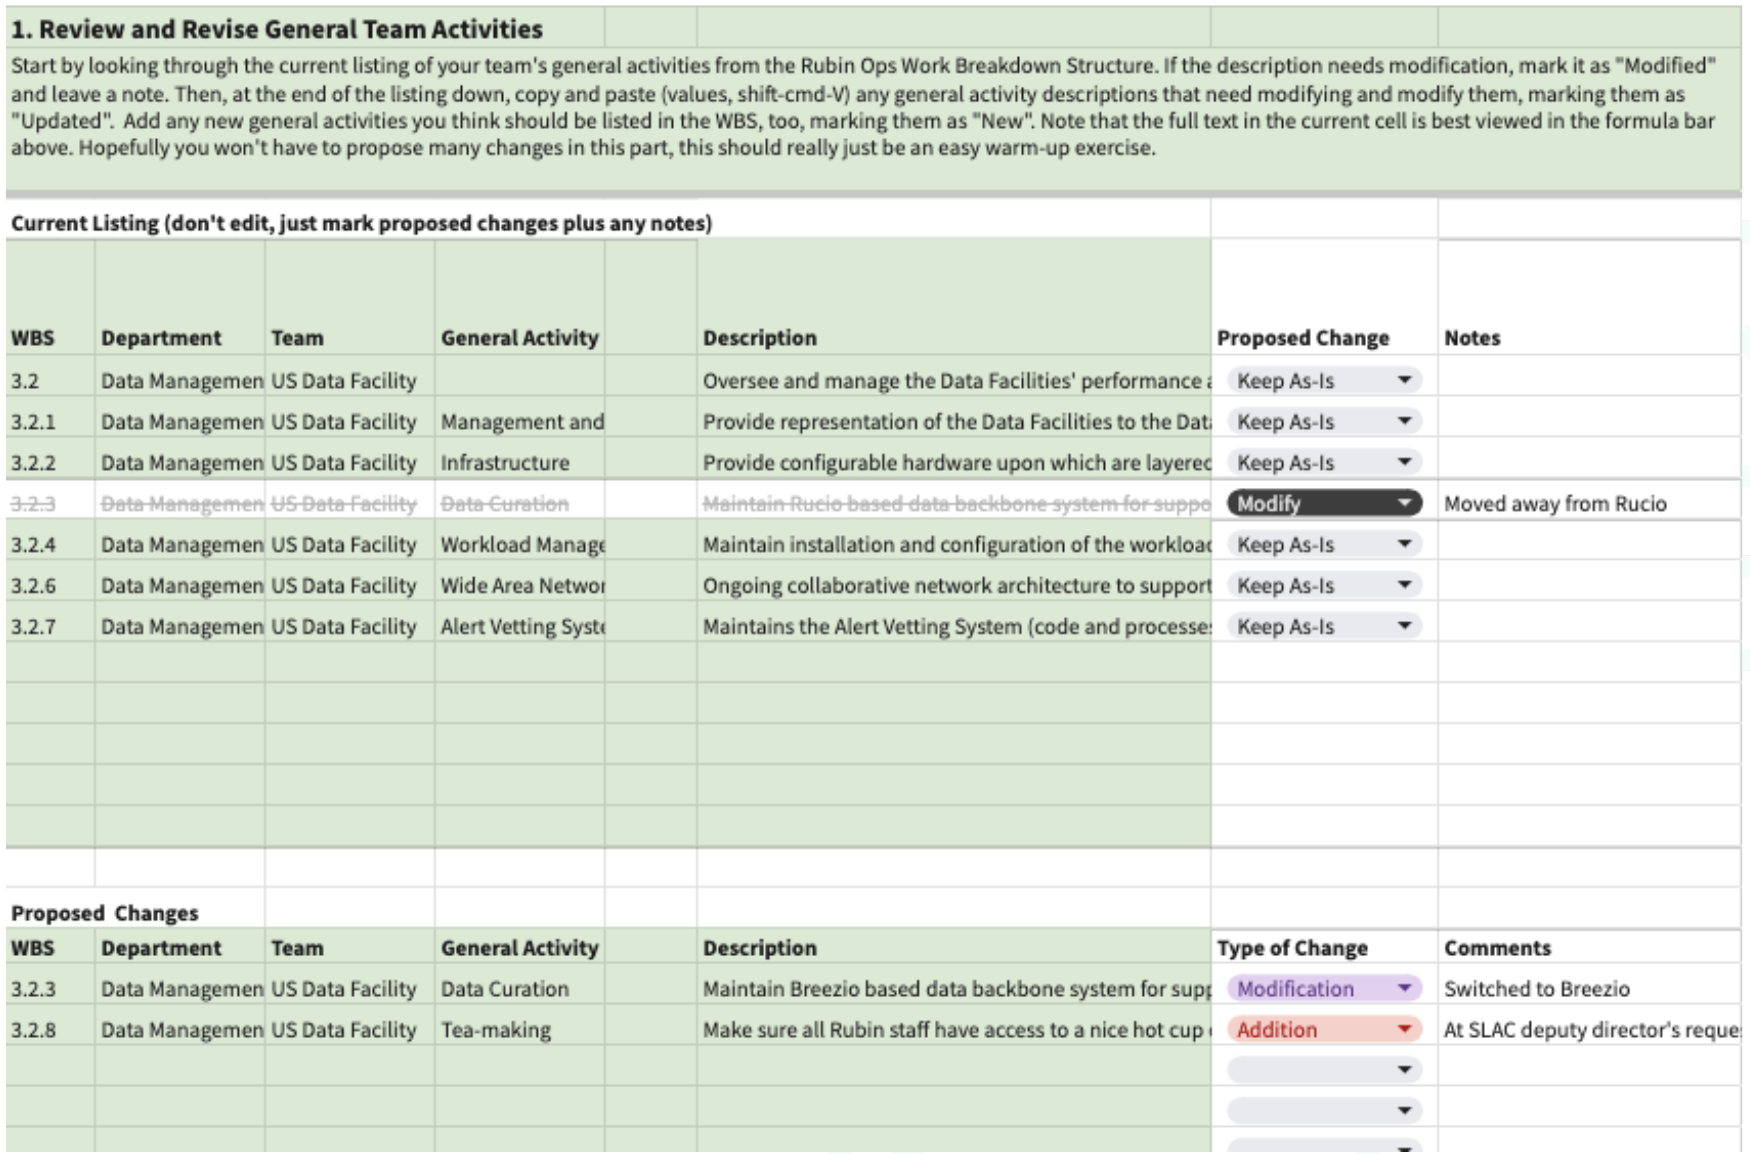
\includegraphics[width=1.0\textwidth]{Figure4WorkBreakdownStructurescrubbing}
	\caption{ Work Breakdown Structure scrubbing
\label{fig:wbs}}
\end{centering}
\end{figure}

\begin{figure}[hb!]
\begin{centering}
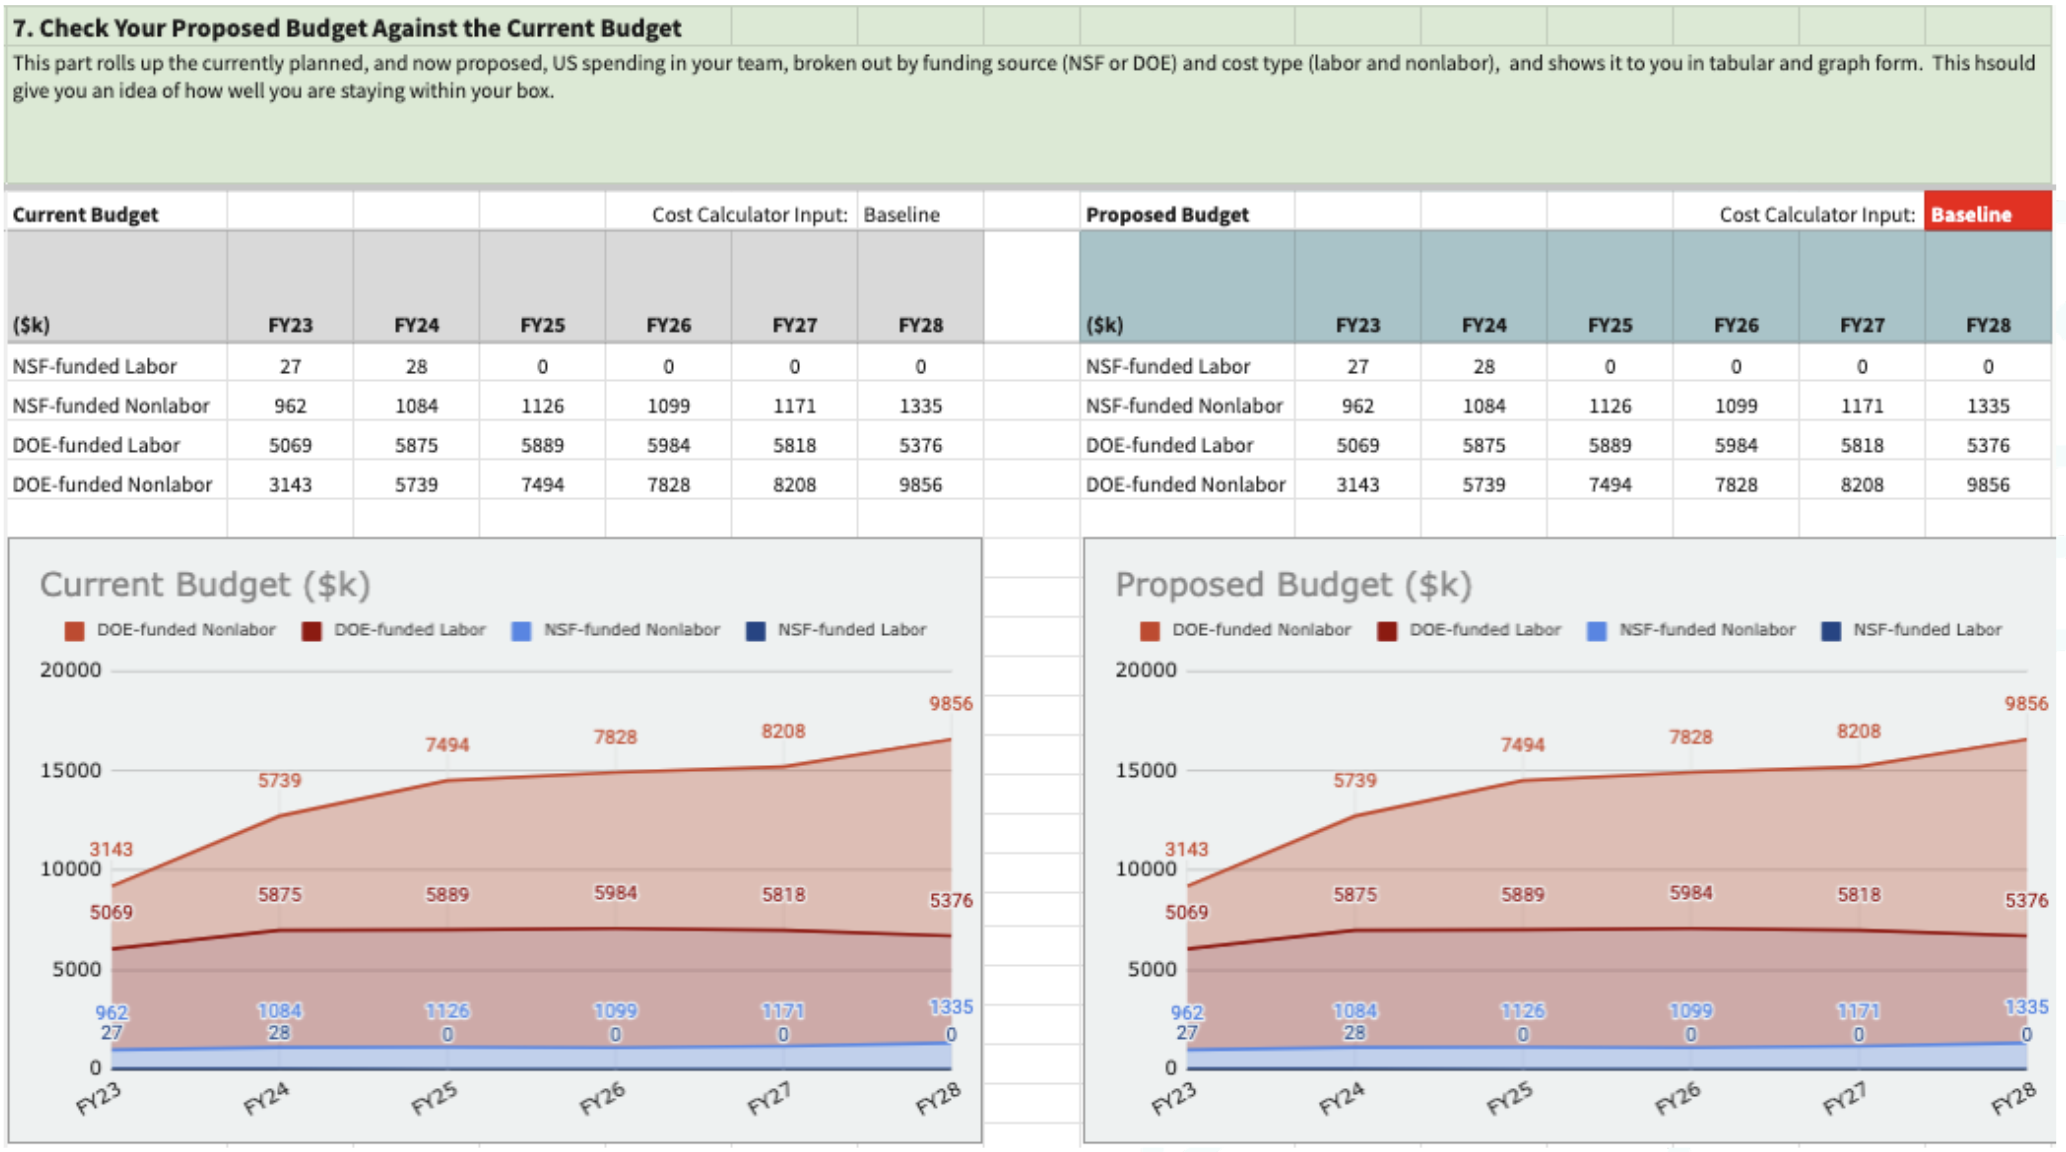
\includegraphics[width=1.0\textwidth]{Figure5BaselinevsProposed}
	\caption{Baseline vs Proposed labor and non-labor comparison
\label{fig:baseline}}
\end{centering}
\end{figure}

\section{Outcomes and Conclusions} \label{sec:outcomes}

This annual iterative process enables change to happen in a controlled and transparent manner, enabling buy-in at all levels on a) what the upcoming FY priorities are and b) the reasons behind difficult decisions which are often inevitable. 
It should be noted that changes can still happen throughout the year through a process called Request Beyond Target (RBT), which enables team leads to request mid-year enhancements to their programs. 
This process is outside of the scope of this paper, but is mentioned here to stress the agile nature of planning at Rubin.

Year on year, as this process takes place from now through to the end of the ten-year Legacy Survey of Space and Time expected in 2037, the scrub process is envisaged to evolve.
ach iteration is expected to reveal gaps and areas of improvement that can be fed into the design of the process and the tools for the following fiscal year’s scrub.





\acknowledgments
This material or work is supported in part by the National Science Foundation through Cooperative Agreement AST-1258333 and Cooperative Support Agreement AST1836783 managed by the Association of Universities for Research in Astronomy (AURA), and the Department of Energy under Contract No. DE-AC02-76SF00515 with the SLAC National Accelerator Laboratory managed by Stanford University.

% Include all the relevant bib files.
% https://lsst-texmf.lsst.io/lsstdoc.html#bibliographies
\bibliographystyle{spiebib}
\bibliography{local,lsst,lsst-dm,refs_ads,refs,books}

% Make sure lsst-texmf/bin/generateAcronyms.py is in your path
\section*{Acronyms} \label{sec:acronyms}
\input{acronyms.tex}


\end{document}
